% Options for packages loaded elsewhere
\PassOptionsToPackage{unicode}{hyperref}
\PassOptionsToPackage{hyphens}{url}
%
\documentclass[
]{article}
\usepackage{amsmath,amssymb}
\usepackage{iftex}
\ifPDFTeX
  \usepackage[T1]{fontenc}
  \usepackage[utf8]{inputenc}
  \usepackage{textcomp} % provide euro and other symbols
\else % if luatex or xetex
  \usepackage{unicode-math} % this also loads fontspec
  \defaultfontfeatures{Scale=MatchLowercase}
  \defaultfontfeatures[\rmfamily]{Ligatures=TeX,Scale=1}
\fi
\usepackage{lmodern}
\ifPDFTeX\else
  % xetex/luatex font selection
\fi
% Use upquote if available, for straight quotes in verbatim environments
\IfFileExists{upquote.sty}{\usepackage{upquote}}{}
\IfFileExists{microtype.sty}{% use microtype if available
  \usepackage[]{microtype}
  \UseMicrotypeSet[protrusion]{basicmath} % disable protrusion for tt fonts
}{}
\makeatletter
\@ifundefined{KOMAClassName}{% if non-KOMA class
  \IfFileExists{parskip.sty}{%
    \usepackage{parskip}
  }{% else
    \setlength{\parindent}{0pt}
    \setlength{\parskip}{6pt plus 2pt minus 1pt}}
}{% if KOMA class
  \KOMAoptions{parskip=half}}
\makeatother
\usepackage{xcolor}
\usepackage[margin=1in]{geometry}
\usepackage{longtable,booktabs,array}
\usepackage{calc} % for calculating minipage widths
% Correct order of tables after \paragraph or \subparagraph
\usepackage{etoolbox}
\makeatletter
\patchcmd\longtable{\par}{\if@noskipsec\mbox{}\fi\par}{}{}
\makeatother
% Allow footnotes in longtable head/foot
\IfFileExists{footnotehyper.sty}{\usepackage{footnotehyper}}{\usepackage{footnote}}
\makesavenoteenv{longtable}
\usepackage{graphicx}
\makeatletter
\newsavebox\pandoc@box
\newcommand*\pandocbounded[1]{% scales image to fit in text height/width
  \sbox\pandoc@box{#1}%
  \Gscale@div\@tempa{\textheight}{\dimexpr\ht\pandoc@box+\dp\pandoc@box\relax}%
  \Gscale@div\@tempb{\linewidth}{\wd\pandoc@box}%
  \ifdim\@tempb\p@<\@tempa\p@\let\@tempa\@tempb\fi% select the smaller of both
  \ifdim\@tempa\p@<\p@\scalebox{\@tempa}{\usebox\pandoc@box}%
  \else\usebox{\pandoc@box}%
  \fi%
}
% Set default figure placement to htbp
\def\fps@figure{htbp}
\makeatother
\ifLuaTeX
  \usepackage{luacolor}
  \usepackage[soul]{lua-ul}
\else
  \usepackage{soul}
\fi
\setlength{\emergencystretch}{3em} % prevent overfull lines
\providecommand{\tightlist}{%
  \setlength{\itemsep}{0pt}\setlength{\parskip}{0pt}}
\setcounter{secnumdepth}{5}
\usepackage{graphicx}
\usepackage{float}
\usepackage{array}
\usepackage{bookmark}
\IfFileExists{xurl.sty}{\usepackage{xurl}}{} % add URL line breaks if available
\urlstyle{same}
\hypersetup{
  pdfauthor={Tom Stuckey},
  hidelinks,
  pdfcreator={LaTeX via pandoc}}

\title{Using SVMs to Classify Activities\\
Report}
\author{Tom Stuckey}
\date{17 Nov 2020}

\begin{document}
\maketitle

\section{Introduction}\label{introduction}

Support Vector Machines (SVMs) are powerful classification and
regression algorithms that work on a wide variety of problem sets. This
effort looks at how SVMs perform on a multi-dimensional, multi-class
classification problem of human activities based on imprecise
radio-frequency identifier (RFID) sensors. This analysis provides the
background of the data, explores the algorithm and its specific
application, provides the results, and discusses the findings.

\subsection{Background and Objective}\label{background-and-objective}

The source data for this effort comes from a 2013 study in Australia
focused on developing a next generation solution for detecting fall risk
in elderly patients in hospital care, residential care, or
rehabilitation centers {[}1{]}. Traditional fall sensors are largely
limited to bed pressure sensors, but they often serve as lagging
indicator for a patient who has already got up and started to move.

The 2013 study looked at using novel passive radio frequency identifiers
(RFID) called Wearable Wireless Identification and Sensing Platform
(WISP) to measure acceleration in three planes of movement in
conjunction with using Conditional Random Fields (CRFs) to classify
movements into four classes of activities: 1. sitting on bed, 2. laying
3. walking, 4, sitting on chair. It included 14 individual patients and
generated over 75,000 individual observations. The data generated from
this study was also submitted to the University of California at Irvine
Machine Learning (UCI ML) repository in 2016 {[}2{]}.

Figure 1 illustrates the sensor and its axes as well as a subject
wearing the sensor {[}1{]}, and Table 1 provides the mapping of the
sensor axes labels used in the source data to the labels used in this
analysis for the sake of clarity.

\begin{figure}
\centering
\pandocbounded{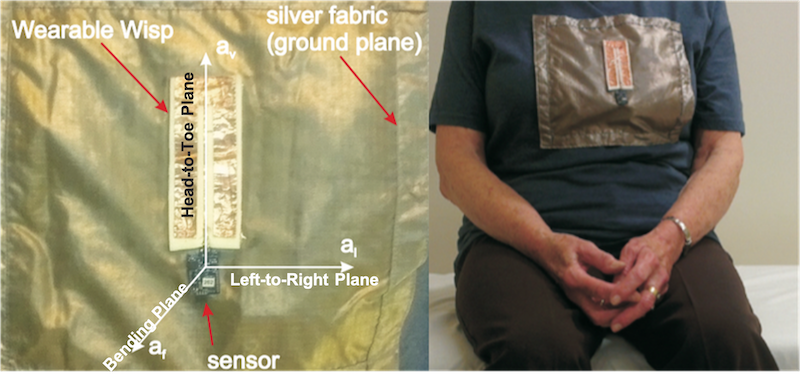
\includegraphics[keepaspectratio]{'./notebooks/R_Notebooks/images/Sensor Illustration.png'}}
\caption{`Sensor Illustration'}
\end{figure}

\begin{longtable}[]{@{}lll@{}}
\caption{Table 1 Axes Enumeration}\tabularnewline
\toprule\noalign{}
Sensor Axes & Axes Relative to Person & Axes in Graphs \\
\midrule\noalign{}
\endfirsthead
\toprule\noalign{}
Sensor Axes & Axes Relative to Person & Axes in Graphs \\
\midrule\noalign{}
\endhead
\bottomrule\noalign{}
\endlastfoot
\(a_l\) & Left-to-Right Plane & x-axis \\
\(a_f\) & Bending Plane & y-axis \\
\(a_v\) & Head-to-Toe Plane & z-axis \\
\end{longtable}

This analysis leverages the 2013 study's labeled data to examine the
effectiveness of Support Vector Machines (SVMs) in successfully classify
activities with the fundamental hypothesis that SVMs can provide a
robust methodology to classify patient activities.

\subsection{Layout}\label{layout}

Section 1 provides the introduction and background of the problem space.
Section 2 describes the methodology employed. Section 3 shows the
results of the analysis. Section 4 discusses the results of the
analysis. Section 5 provides a summary and conclusion. Section 6 lists
the references.

\newpage

\section{Method}\label{method}

This section provides a brief overview the pre-processing routines and
the support vector classification methodology used.

\subsection{Pre-Processing and
Accuracy}\label{pre-processing-and-accuracy}

\subsubsection{Transformations}\label{transformations}

To enable this analysis, several pre-processing routines were employed.
First, the source data from the 2013 study is hosted on the UCI ML
repository website as an archive of 94 separate files with important
features embedded in both the directory structure the file names
themselves. Leveraging a dynamic approach, the data is imported into the
R runtime as a tibble data structure and key features from the directory
structure and file names are added as columns. Second, balancing the
goals of cross-validated model development (described below) and
challenges with applying a binary learner to a multi-class data set, the
data is broken into five partitions using the same class distribution as
the full data set. Third, for each partition, one-vs-all encoding is
applied with several manipulations such that for each positive activity,
all other activities are marked as negative. Last, the five partitions
with the one-vs-all encoding markers are rejoined into a single, revised
data structure such that filtering on a single data structure enables
the analysis based on stratification group and positive activity class.

\subsubsection{Cross Validation}\label{cross-validation}

Aligned with the one-vs-all encoding and stratification strategy
described above, a simple, five fold cross-validation scheme is
leveraged. For each stratified partition, each of the four activities:
``Sitting on Bed'', ``Laying,'' ``Walking,'' and ``Sitting on Chair'' is
held out at the positive activity. Then, that partition is further
broken into a stratified 70\%/30\%, training/testing split. For each
activity in each partition, a model is built with the training data,
predictions are made with the model using the test data, and the
accuracy is recorded. The model, test data, and accuracy are recorded,
and the best performing model across all partitions for each activity
class is retained.

\subsubsection{Accuracy}\label{accuracy}

Accuracy for this analysis is computed in the usual way for with a
confusion matrix as illustrated in figure 2. Accuracy is computed as the
sum true positive and true negative classifications divided by the total
number of classifications.

\begin{figure}[H]
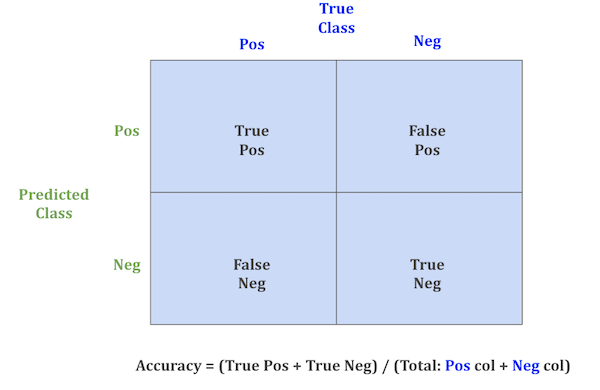
\includegraphics[width=0.5\linewidth]{./notebooks/R_Notebooks/images/Accuracy} \caption{Accuracy}\label{fig:accuracy}
\end{figure}

\subsection{Support Vector Machine
Classification}\label{support-vector-machine-classification}

Support Vector Machines (SVMs) are a useful type of linear machine
learning algorithm that is particularly resilient and effective for
classification and regression tasks in both low and high-dimensional
datasets. The following subsection provide a brief history of SVMs and
how they enable this classification based analysis.

\subsubsection{Support Vector Machines Brief
History}\label{support-vector-machines-brief-history}

SVMs lineage can be traced back to Ron Fisher's Linear Discriminate
Analysis in the 1930s. However, the general SVM algorithm is more
directly related to work of Vapnik and Chervonenkis in their
\emph{Theory of Pattern Recognition} in 1974 {[}8{]}, and the 1992 paper
\emph{A Training Algorithm for Optimal Margin Classifiers {[}3{]}}
formalized maximal margin classifiers. These maximal margin classifiers
generalize first as two-dimensional support vector classifiers and in
n-dimensions as SVMs. Stated plainly, SVMs follow a straightforward
pattern: 1. Start with data in a low dimension, 2. Move that data to a
higher dimension, 3. Find a support vector classifier to separate the
higher dimensional data into two groups {[}4{]}.

The particular mechanism to do approximate this higher dimension
movement is to leverage a construct known as \textbf{the kernel trick}.
By computing a dot product between vectors (the projection of one vector
onto another) in the original space and raising the scalar result to a
power, it is functionally the same as computing the dot product in a
higher order space {[}9{]}. Popular kernels for this include the linear,
polynomial, radial basis function, and sigmoid variants.

\subsubsection{Support Vector Machines
Applied}\label{support-vector-machines-applied}

For this analysis, the SVM component of e1071 R package {[}10{]} is
leveraged. Building from previous experiences, the radial basis function
provides strong performance and is therefore used in this analysis. As a
reminder, the \textbf{radial basis function} is\textbf{:} \[
e ^ { -\gamma || \boldsymbol{u} - \boldsymbol{v}||_2} 
\]

Where \textbf{u} and \textbf{v} represent any two dimensions in the
problem space, and, as is proven in {[}11{]}, this euclidean norm maps
into infinite dimensions.

Some additional parameters specified include the \(\gamma\) value, which
determines how quickly the class boundaries dissipate beyond the support
vectors, and the \textbf{cost}, which as a penalty factor for
misclassifying a point. Accordingly, the specific call to build the
model in this analysis is:

\begin{verbatim}
my_model <- e1071::svm(activity_class ~ bending + head_to_toe + left_to_right + signal_strength, 
data = train_df, kernel = 'radial', gamma = 5, cost = 25, scale = FALSE)
\end{verbatim}

\newpage

\section{Analysis}\label{analysis}

Aligned with the methodology described in section 2, this section
provides the results of the SVM-based analysis. It begins with the
summary performance information and then provides the predictions using
the best model for each activity.

\subsection{Summary Performance
Measures}\label{summary-performance-measures}

Table 2 shows the raw accuracy metrics for each activity for each
stratification. Within each stratification group, the best performing
group is \ul{\textbf{emboldened and underlined}}.

\begin{longtable}[]{@{}
  >{\raggedright\arraybackslash}p{(\linewidth - 4\tabcolsep) * \real{0.4143}}
  >{\raggedright\arraybackslash}p{(\linewidth - 4\tabcolsep) * \real{0.3143}}
  >{\raggedright\arraybackslash}p{(\linewidth - 4\tabcolsep) * \real{0.2714}}@{}}
\caption{Summary Accuracy Across Stratified Groups}\tabularnewline
\toprule\noalign{}
\begin{minipage}[b]{\linewidth}\raggedright
Activity
\end{minipage} & \begin{minipage}[b]{\linewidth}\raggedright
Stratification Group
\end{minipage} & \begin{minipage}[b]{\linewidth}\raggedright
Accuracy
\end{minipage} \\
\midrule\noalign{}
\endfirsthead
\toprule\noalign{}
\begin{minipage}[b]{\linewidth}\raggedright
Activity
\end{minipage} & \begin{minipage}[b]{\linewidth}\raggedright
Stratification Group
\end{minipage} & \begin{minipage}[b]{\linewidth}\raggedright
Accuracy
\end{minipage} \\
\midrule\noalign{}
\endhead
\bottomrule\noalign{}
\endlastfoot
Sitting on Bed & 1 & 94.532\% \\
Sitting on Bed & 2 & 94.426\% \\
Sitting on Bed & 3 & 94.142\% \\
Sitting on Bed & 4 & 94.568\% \\
\ul{\textbf{Sitting on Bed}} & \ul{\textbf{5}} &
\ul{\textbf{94.71\%}} \\
Laying & 1 & 99.627\% \\
\ul{\textbf{Laying}} & \ul{\textbf{2}} & \ul{\textbf{99.73\%}} \\
Laying & 3 & 99.645\% \\
Laying & 4 & 99.663\% \\
Laying & 5 & 99.645\% \\
Walking & 1 & 98.296\% \\
Walking & 2 & 98.42\% \\
Walking & 3 & 98.242\% \\
\ul{\textbf{Walking}} & \ul{\textbf{4}} & \ul{\textbf{98.72\%}} \\
Walking & 5 & 98.385\% \\
Sitting on Chair & 1 & 96.023\% \\
Sitting on Chair & 2 & 96.059\% \\
Sitting on Chair & 3 & 95.651\% \\
Sitting on Chair & 4 & 95.899\% \\
\ul{\textbf{Sitting on Chair}} & \ul{\textbf{5}} &
\ul{\textbf{96.11\%}} \\
\end{longtable}

\newpage

\subsection{Predictions}\label{predictions}

The following sub-sections contain graphical illustrations of the
predictions and errors of the best model for each activity. As a recap,
each model is built using a one-vs-all approach where activities are
either in the positive class or out of the positive class. Additionally,
for this study the three most operationally important features are the
three planes of patient movement. This means the ideal graphical
rendering should depict all three planes of movement instead of applying
any dimensionality reduction techniques. Accordingly, for each of the
following sub-sections, in the 2D graph, the x-axis represents the
Left-to-Right Acceleration, the y-axis represents the Bending
Acceleration, and the z-axis represents the Head-to-Toe Acceleration as
depicted by the size of the plotted point. Red dots denote negative
class membership, and turquoise dots denote positive class membership.
Dot opacity is set to 50\% to better indicate when multiple dots
overlap. Misclassified points are indicated with a blue X over the
point.

\subsubsection{Predictions for Sitting on
Bed}\label{predictions-for-sitting-on-bed}

Figure 3 provides a graphical rendering of the model with the positive
class ``Sitting on Bed.'' Stratification group 5 provided the most
accurate model for ``Sitting on Bed'' where it was 94.71\% accurate
across the test data for stratification group 5.

\begin{figure}[H]
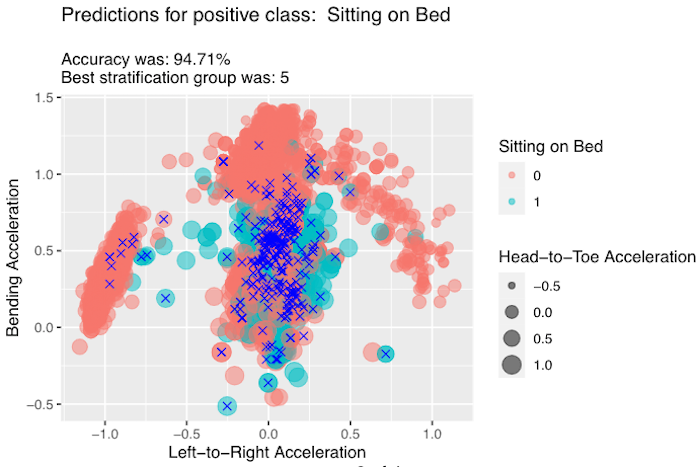
\includegraphics[width=0.75\linewidth]{./notebooks/R_Notebooks/images/Sitting on Bed Predictions} \caption{Sitting on Bed Predictions}\label{fig:sitting on bed results}
\end{figure}

\newpage

\subsubsection{Predictions for Laying}\label{predictions-for-laying}

Figure 4 provides a graphical rendering of the model with the positive
class ``Laying'' Stratification group 2 provided the most accurate model
for ``Laying where it was 99.73\% accurate across the test data for
stratification group 2.

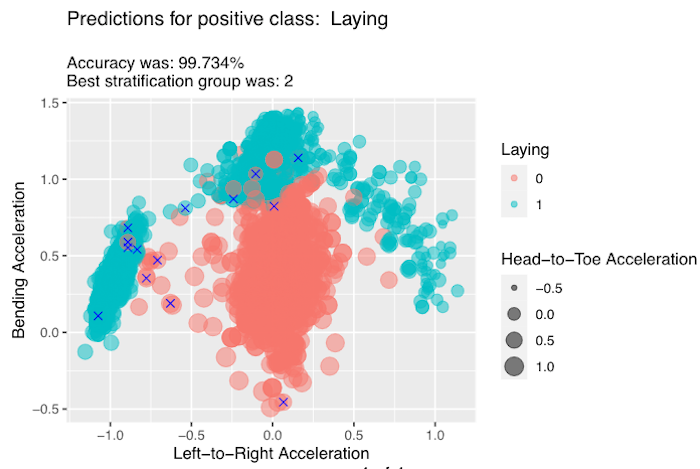
\includegraphics[width=0.75\linewidth]{./notebooks/R_Notebooks/images/Laying Predictions}

\subsubsection{Predictions for Walking}\label{predictions-for-walking}

Figure 5 provides a graphical rendering of the model with the positive
class ``Walking'' Stratification group 4 provided the most accurate
model for ``Laying where it was 98.72\% accurate across the test data
for stratification group 4.

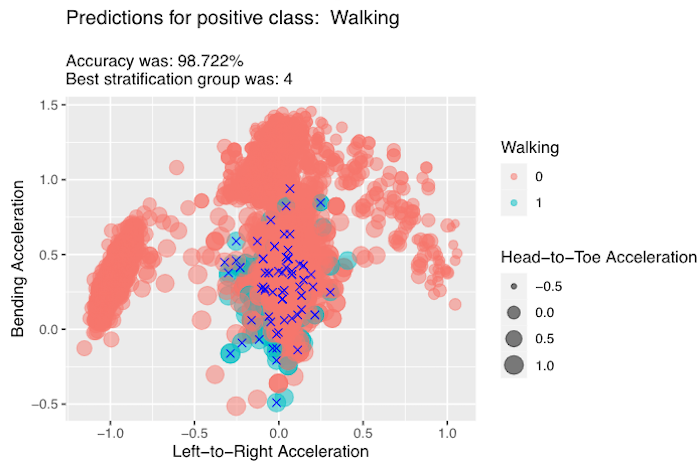
\includegraphics[width=0.75\linewidth]{./notebooks/R_Notebooks/images/Walking Predictions}

\subsubsection{Predictions for Sitting on
Chair}\label{predictions-for-sitting-on-chair}

Figure 6 provides a graphical rendering of the model with the positive
class ``Walking'' Stratification group 5 provided the most accurate
model for ``Laying where it was 96.12\% accurate across the test data
for stratification group 5.

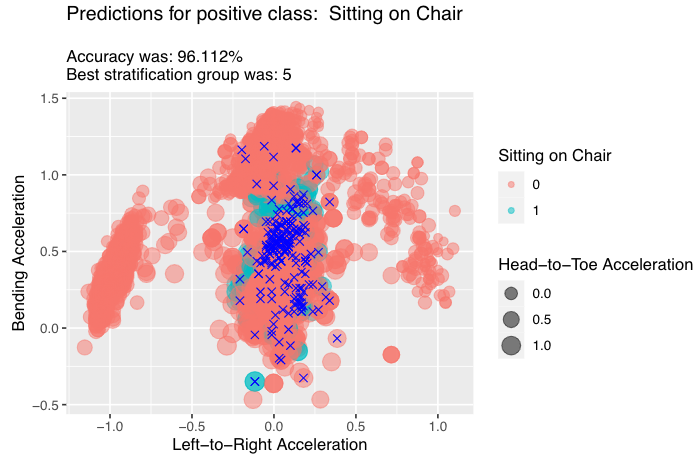
\includegraphics[width=0.75\linewidth]{./notebooks/R_Notebooks/images/Sitting on Chair Predictions}

\newpage

\section{Discussion}\label{discussion}

Section 4 provides accuracy measurements for activities and
stratification groups and provides illustrations for the best models for
each activity. At face value, the classifications have remarkable
accuracy ranging from low of 94.71\% for the ``Sitting on Bed'' class to
a high of 99.73\% for the ``Laying'' class. The stratification routine
applied during transformation (as described in Section 2) minimizes
overfitting (due to distribution aligned sampling), and the
cross-validation routine (also described in Section 2) builds and
analyzes five individual models per activity class. Accordingly, this
appears to be a robust analysis with colloquially ``good'' accuracy
across the board. The follow sub-sections provide discuss some potential
shortfalls and some considerations for future analysis.

\subsection{Potential Shortfalls}\label{potential-shortfalls}

A significant potential shortfall for discussion is the small sample
size and the lack of any time series analysis. As mentioned briefly
mentioned in Section 1, there were 14 individual patients in the scope
of the 2013 study that generated the 75,000+ observations leveraged in
this analysis. Consecutive recording intervals from each RFID sensor
ranged from 0.025 sec to 10 sec {[}1{]}; however, the approach employed
in this analysis treats each observation as independent when they may
not be. Future analysis could potentially further transform the data
with additional features to mitigate actual dependence between
consecutive observations; an approach to this is described in SVM
Kernels for Time Series Analysis {[}5{]}.

In retrospect, some inductive bias is likely introduced by radio
frequency (RF) ignorance may have degraded the quality of the analysis.
Inductive bias refers to assumptions about the transformation function
that extends beyond the training data {[}8{]}. In this case, the
inclusion of signal strength in model generation with the thought it
would more strongly weight correct classifications was a heuristic and
not based on deep analysis of RF and signal processing.

\subsection{Future Analysis}\label{future-analysis}

Additional analysis could be performed on different room configurations.
The source study employed two different room configurations, however, in
this analysis, the room identifier is excluded from the SVM model
construction. Future efforts could include more rigorous analysis of
different room configurations to evaluate the model accuracy from one
room configuration to another, or they might include AB Tests {[}6{]}
between the two rooms using the existing configuration agnostic models
to identify the better sensor configuration.

Another potential area for future analysis could be to explicitly
examine outliers. By design, SVM analysis excludes the outliers, but
meaningful analysis of outliers could yield additional insights. For
example it could identify additional data correlations. \emph{Outlier
Analysis} {[}7{]} provides several strategies for both time-series and
linear discriminant (the parent family of SVM)-based analysis.

\newpage

\section{Conclusion}\label{conclusion}

This report has provided an overview of the problem space, presented a
hypothesis SVMs can provide a robust solution, walked through the basic
mechanics of SVMs, and presented the analysis with discussion. To close,
one question that may come up is ``how does one use these models in real
time in a real world setting?'' The answer is to run each observation
through all the models in a nested fashion. For example, given a single
observation such as in Table 3:

\begin{longtable}[]{@{}
  >{\raggedright\arraybackslash}p{(\linewidth - 20\tabcolsep) * \real{0.0635}}
  >{\raggedright\arraybackslash}p{(\linewidth - 20\tabcolsep) * \real{0.0714}}
  >{\raggedright\arraybackslash}p{(\linewidth - 20\tabcolsep) * \real{0.1032}}
  >{\raggedright\arraybackslash}p{(\linewidth - 20\tabcolsep) * \real{0.1190}}
  >{\raggedright\arraybackslash}p{(\linewidth - 20\tabcolsep) * \real{0.0873}}
  >{\raggedright\arraybackslash}p{(\linewidth - 20\tabcolsep) * \real{0.1349}}
  >{\raggedright\arraybackslash}p{(\linewidth - 20\tabcolsep) * \real{0.0635}}
  >{\raggedright\arraybackslash}p{(\linewidth - 20\tabcolsep) * \real{0.0873}}
  >{\raggedright\arraybackslash}p{(\linewidth - 20\tabcolsep) * \real{0.0794}}
  >{\raggedright\arraybackslash}p{(\linewidth - 20\tabcolsep) * \real{0.0635}}
  >{\raggedright\arraybackslash}p{(\linewidth - 20\tabcolsep) * \real{0.1270}}@{}}
\caption{Exemplar Observation}\tabularnewline
\toprule\noalign{}
\begin{minipage}[b]{\linewidth}\raggedright
time
\end{minipage} & \begin{minipage}[b]{\linewidth}\raggedright
bending
\end{minipage} & \begin{minipage}[b]{\linewidth}\raggedright
head\_to\_toe
\end{minipage} & \begin{minipage}[b]{\linewidth}\raggedright
left\_to\_right
\end{minipage} & \begin{minipage}[b]{\linewidth}\raggedright
sensor\_id
\end{minipage} & \begin{minipage}[b]{\linewidth}\raggedright
signal\_strength
\end{minipage} & \begin{minipage}[b]{\linewidth}\raggedright
phase
\end{minipage} & \begin{minipage}[b]{\linewidth}\raggedright
frequency
\end{minipage} & \begin{minipage}[b]{\linewidth}\raggedright
location
\end{minipage} & \begin{minipage}[b]{\linewidth}\raggedright
gender
\end{minipage} & \begin{minipage}[b]{\linewidth}\raggedright
activity\_class
\end{minipage} \\
\midrule\noalign{}
\endfirsthead
\toprule\noalign{}
\begin{minipage}[b]{\linewidth}\raggedright
time
\end{minipage} & \begin{minipage}[b]{\linewidth}\raggedright
bending
\end{minipage} & \begin{minipage}[b]{\linewidth}\raggedright
head\_to\_toe
\end{minipage} & \begin{minipage}[b]{\linewidth}\raggedright
left\_to\_right
\end{minipage} & \begin{minipage}[b]{\linewidth}\raggedright
sensor\_id
\end{minipage} & \begin{minipage}[b]{\linewidth}\raggedright
signal\_strength
\end{minipage} & \begin{minipage}[b]{\linewidth}\raggedright
phase
\end{minipage} & \begin{minipage}[b]{\linewidth}\raggedright
frequency
\end{minipage} & \begin{minipage}[b]{\linewidth}\raggedright
location
\end{minipage} & \begin{minipage}[b]{\linewidth}\raggedright
gender
\end{minipage} & \begin{minipage}[b]{\linewidth}\raggedright
activity\_class
\end{minipage} \\
\midrule\noalign{}
\endhead
\bottomrule\noalign{}
\endlastfoot
136.38 & 0.24858 & 0.33072 & -1.0172 & 2 & -49 & 2.4866 & 921.25 & two &
female & 3 \\
\end{longtable}

Running this sample row through all four models, one can see that the
model for the positive class ``Laying'' (activity class 3) was the one
predicted positive:

\begin{verbatim}
For actual: Laying:
     predicted WAS NOT Sitting on Bed 
     predicted WAS Laying 
     predicted WAS NOT Walking 
     predicted WAS NOT Sitting on Chair 
\end{verbatim}

Ties could either be mitigated by stopping at the first positive
classification or by random draw of all positive classes returned.
Circling back, one may also question why this single example is held out
as an operational example; after all, a much more thorough accuracy
analysis was presented in Section 3. This example emphasizes the how the
model could be used in a real environment whereas the accuracy measures
from Section 3 are to empirically assess accuracy on large existing data
sets.

This effort demonstrates that SVMs can classify patient activities with
high accuracy using data from low-cost, low-maintenance, non-restricting
RIFD sensors. Clearly, this provides evidence that SVM-based classifying
algorithms could be a key solution component to a big problem space in
hospital care, residential care, or rehabilitation centers.

\newpage

\section{References}\label{references}

{[}1{]} Torres, R. L. S., Ranasinghe, D. C., Shi, Q., \& Sample, A. P.
(2013, April). Sensor enabled wearable RFID technology for mitigating
the risk of falls near beds. In 2013 IEEE International Conference on
RFID (RFID) (pp.~191-198). IEEE.

{[}2{]} Torres, R. L. S. T., Ranasinghe, D. R., \& Visvanathan, R. V.
(2016). Activity recognition with healthy older people using a
batteryless wearable sensor Data Set. UCI Machine Learning.
\url{https://archive.ics.uci.edu/ml/datasets/Activity+recognition+with+healthy+older+people+using+a+batteryless+wearable+sensor}

{[}3{]} Boser, B. E., Guyon, I. M., \& Vapnik, V. N. (1992, July). A
training algorithm for optimal margin classifiers. In Proceedings of the
fifth annual workshop on Computational learning theory (pp.~144-152).

{[}4{]} StatQuest with Josh Starmer. (2019, September 30). Support
Vector Machines, Clearly Explained!!! YouTube.
\url{https://www.youtube.com/watch?v=efR1C6CvhmE}

{[}5{]} Rüping, S. (2001). \emph{SVM kernels for time series analysis}
(No.~2001, 43). Technical report.

{[}6{]} STAT 88. (n.d.). \emph{A/B Testing: Fisher's Exact Test}. STAT
88.Org. Retrieved November 14, 2020, from
\url{http://stat88.org/textbook/notebooks/Chapter_09/02_AB_Testing_Fishers_Exact_Test.html}

{[}7{]} Aggarwal, C. C. (2016). \emph{Outlier Analysis} (2nd ed.~2017
ed.). Springer.

{[}8{]} Hamilton, L. H. (2014, October 1). \emph{The Inductive Biases of
Various Machine Learning Algorithms}. Lauradhamilton.Com.
\url{http://www.lauradhamilton.com/inductive-biases-various-machine-learning-algorithms}

{[}8{]} Vapnik, V. N., \& Chervonenkis, A. (1974). Theory of pattern
recognition, 1974. \emph{Russian}.

{[}9{]} Ranjan, C. R. (2019, May 9). \emph{Understanding the Kernel
Trick with fundamentals}. Towards Data Science.
\url{https://towardsdatascience.com/truly-understanding-the-kernel-trick-1aeb11560769}

{[}10{]} \emph{e1071} (1.7-4). (2020). {[}Misc Functions of the
Department of Statistics, Probability Theory Group{]}. CRAN.
\url{https://cran.r-project.org/web/packages/e1071/index.html}

{[}11{]} University of Wisconsin. (n.d.). \emph{The Radial Basis
Function Kernel}. Cs.Wisc.Edu. Retrieved November 14, 2020, from
\url{http://pages.cs.wisc.edu/~matthewb/pages/notes/pdf/svms/RBFKernel.pdf}

\end{document}
